\documentclass[a4paper,11pt]{article}

% 日本語対応
\usepackage{xeCJK}
\setCJKmainfont{Yu Gothic}

% 数学関連パッケージ
\usepackage{amsmath}
\usepackage{amssymb}
\usepackage{amsthm}
\usepackage{amsfonts}
\usepackage{mathtools}

% 図形描画用パッケージ
\usepackage{tikz}
\usepackage{pgfplots}
\pgfplotsset{compat=1.18}
\usetikzlibrary{intersections,patterns,angles,quotes,calc,fillbetween}

% その他パッケージ
\usepackage{graphicx}
\usepackage{enumitem}
\usepackage{float}
\usepackage{hyperref}
\usepackage{fancyhdr}
\usepackage{geometry}
\usepackage{xcolor}

% ページ設定
\geometry{
  a4paper,
  top=25mm,
  bottom=25mm,
  left=25mm,
  right=25mm
}

% 数式環境設定
\numberwithin{equation}{section}
\newtheorem{theorem}{定理}
\newtheorem{lemma}[theorem]{補題}
\newtheorem{proposition}[theorem]{命題}
\newtheorem{corollary}[theorem]{系}
\theoremstyle{definition}
\newtheorem{definition}[theorem]{定義}
\newtheorem{example}[theorem]{例}
\newtheorem{exercise}{問題}
\theoremstyle{remark}
\newtheorem*{remark}{注意}
\newtheorem*{solution}{解答}

% ヘッダーとフッターの設定
\pagestyle{fancy}
\fancyhf{}
\fancyhead[L]{数学問題}
\fancyhead[R]{\today}
\fancyfoot[C]{\thepage}
\renewcommand{\headrulewidth}{0.4pt}
\renewcommand{\footrulewidth}{0.4pt}

% タイトル情報
\title{数学問題}
\author{数学問題生成AIシステム}
\date{\today}

% ドキュメント開始
\begin{document}

\maketitle

% 問題セクション
\section*{問題}

% 問題文を挿入(変数で置換)
2次関数 $f(x) = 3x^2 - 12x + 9$ の頂点の座標を求めるには、まず頂点の公式を使用します。頂点の$x$座標は $x = -\frac{b}{2a}$ で求められます。ここで、$a = 3$、$b = -12$ です。したがって、

$x = -\frac{-12}{2 \cdot 3} = \frac{12}{6} = 2$

次に、この$x$の値を元の関数に代入して$y$の値を求めます。

$f(2) = 3(2)^2 - 12(2) + 9 = 12 - 24 + 9 = -3$

よって、頂点の座標は $(2, -3)$ です。

% 図形が必要な場合はここに挿入
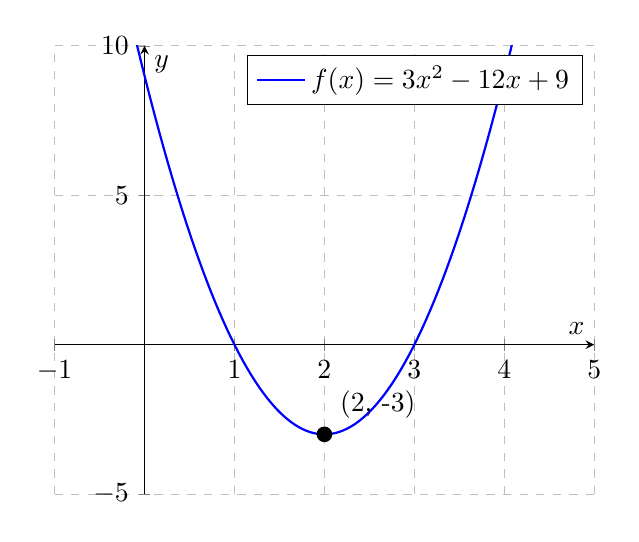
\begin{tikzpicture}
\begin{axis}[
    axis lines=middle,
    xlabel={$x$},
    ylabel={$y$},
    xmin=-1, xmax=5,
    ymin=-5, ymax=10,
    grid=major,
    grid style=dashed,
    ]
    
    % 関数の描画
    \addplot[domain=-1:5, samples=100, smooth, thick, blue] {3*x^2 - 12*x + 9};
    \addlegendentry{$f(x) = 3x^2 - 12x + 9$}
    
    % 頂点の描画
    \node[label={45:{(2, -3)}},circle,fill,inner sep=2pt] at (axis cs:2,-3) {};
    
\end{axis}
\end{tikzpicture}

% 解答セクション(オプショナル - 表示したくない場合はコメントアウト)
\section*{解答}

% 解答を挿入(変数で置換)
LaTeX形式では、点の座標をそのまま記述するだけで十分です。したがって、入力文 "(2, -3)" をLaTeX形式に変換すると、以下のようになります。

```
$(2, -3)$

% 解説セクション(オプショナル - 表示したくない場合はコメントアウト)
\section*{解説}

% 解説を挿入(変数で置換)
2次関数の一般形は $f(x) = ax^2 + bx + c$ である。与えられた関数において、$a = 3$、$b = -12$、$c = 9$ である。2次関数の頂点の座標は $\left(-\frac{b}{2a}, f\left(-\frac{b}{2a}\right)\right)$ で求めることができる。

- まず、$-\frac{b}{2a}$ を計算すると、$-\left(-\frac{12}{2\cdot 3}\right) = \frac{12}{6} = 2$ である。
- 次に、$f(2)$ を計算すると、$f(2) = 3\cdot(2)^2 - 12\cdot 2 + 9 = 3\cdot 4 - 24 + 9 = 12 - 24 + 9 = -3$ である。

したがって、頂点の座標は $(2, -3)$ である。

\end{document} 